La energía nuclear es hoy día imprescindible para proporcionar la potencia eléctrica necesaria en el mundo desarrollado.  Aunque  otras fuentes de energía se están desarrollando a gran velocidad (fotovoltáica, eólica, energía de las mareas), y otros conceptos de producción y ahorro de energía también (producción local, techos solares, eficiencia energética, ciudades inteligentes), es impensable por ahora paralizar la producción de energía nuclear, que proporciona una fuente estable, barata y que no depende de parámetros meteorológicos, y que desde el  punto de vista de emisión de gases de efecto invernadero es relativamente limpia, ya que la única huella de carbono asociada es debida a la minería del uranio y al transporte y reciclaje del combustible.
Los detractores de la energía nuclear argumentan, en cambio, el riesgo de contaminación radiactiva y los accidentes ocurridos en el pasado: Chernobil y Fukushima. Otra razón importante es que las centrales nucleares son una de las raíces de la proliferación nuclear.

Se sea partidario o detractor de la energía nuclear, está claro que la seguridad de las mismas no es un aspecto  negociable y que deben de existir mecanismos que adviertan de cualquier mal funcionamiento de una central nuclear.  Las principales señales de alerta de mal funcionamiento de una central nuclear es la emisión de cantidades anormales de radiactividad. Una central nuclear operando en modo normal puede llegar a emitir alrededor de $300\ \tera\becquerel/\giga\watt\mathrm{y}$ \cite{300TBq}. Como hemos dicho antes, un reactor nuclear se caracteriza por una extremada estabilidad en su funcionamiento, y por ende, en una emisión constante  de isótopos radiactivos.  Cualquier variación de esta tasa de emisión puede ser un indicador de un problema en el reactor o el circuito de refrigeración de mismo. Entre los isótopos radiactivos emitidos por una central  nuclear está el tritio, que se produce mediante captura de neutrones del deuterio presente en el  agua pesada, o doble captura de neutrones del hidrógeno del agua normal, lo cual ocurre con cierta probabilidad debido al enorme flujo de neutrones de un reactor nuclear (del orden de $10^{14} \ce{n} \, \cm^-2\second^-1$).  El tritio se emite como agua tritiada en el agua de refrigeración del circuito secundario  de la central.  

La detección de un exceso de tritio en tiempo cuasi real es esencial por las siguientes razones:

\begin{enumerate}

\item  Advierte de la producción de un exceso de neutrones por el reactor nuclear, o de una fuga de agua de refrigeración del circuito primario. Ambas causas son precursores de problemas que podría a evolucionar, resultando más graves.

\item  El agua de refrigeración del secundario normalmente forma parte de aguas  empleadas posteriormente para la irrigación o el consumo humano. Dado que el límite máximo de actividad de tritio permitida para el consumo humano por la normativa europea  es de $100~\becquerel/\liter$, está claro que  una contaminación de las aguas de refrigeración las convertiría rápidamente en no potables e impediría la consumición de las cosechas afectadas, ya que la vida media del tritio es de unos 12 años.

\item  Muchos de los caudales de agua empleados en la refrigeración de las centrales nucleares, son transfronterizos, es decir, transcurren por dos o más países.  La emisión de tritio en el país propietario de la central nuclear podría causar graves problemas en el país vecino.


\end{enumerate}


Por estas razones, poder medir niveles de tritio en tiempo cuasi-real es de suma importancia en un sistema de vigilancia de una central nuclear. Sin embargo, actualmente ninguna técnica permite medir niveles de actividad de tritio del $\kilo\becquerel$ en tiempos del orden de $15$ minutos.   Se pueden medir actividades  del orden del $\becquerel$  mediante la técnica del centelleo líquido, comentada más adelante, pero requiere tiempos de medida de unos dos días, demasiado largo comparado con el posible ritmo de evolución de un problema en una central nuclear.   Todas estas razones han motivado el proyecto Tritium, con título ``Diseño, construcción y puesta a punto de estaciones automáticas para el monitoraje en tiempo real de bajos niveles radiactivos de tritio en aguas",  financiado por el programa Interreg Sudoe de la CEE en la convocatoria de 2016 con número de referencia  SOE1/P4/E0214", cuya finalidad es desarrollo de un detector de tritio en tiempo cuasi-real basado en la tecnología de fibras centelleadoras leídas por fotomultiplicadores de silicio. Su objetivo es la construcción de un prototipo que sería instalado en el embalse de refrigeración de la central nuclear de Almaraz, en el río Tajo, cuyas aguas se emplean como agua potable en España y Portugal.
La colaboración \textit{Tritium} es un grupo internacional compuesto por 6 centros de tres países:  La Universidad de Aveiro de Portugal,  la Universidad de Burdeos y el CNRS (Section Aquitaine-Limousin)  de Francia y  la Universidad de Extremadura, la Junta de Extremadura y la Universidad de Valencia de España. El proyecto \textit{Tritium} es  obviamente demasiado extenso como trabajo de fin de máster ya que  su ejecución se prolonga durante tres  años  y será la base de mi futura Tesis Doctoral. En este trabajo de fin de máster únicamente nos centraremos en los primeros pasos de este gran proyecto, el cual ha empezado recientemente y, afortunadamente, me ha permitido estar en este desde el inicio.









La creación de altos niveles de tritio es un problema que concierne no sólo a  a las  centrales nucleares de fisión sino también a las  futuras centrales de fusión termonuclear y reactores nucleares experimentales. Algunos experimentos científicos emplean elevadas cantidades de tritio.

\subsection{Propiedades del tritio}

El tritio  es el tercer isótopo de hidrógeno formado por un protón y dos neutrones. Algunos de los principales canales de producción de tritio son la captura neutrónica del $\ce{D}$, $\ce{^6Li}$, $\ce{^7Li}$,  las cuales se muestran a continuación:
\begin{equation}
\ce{^{6}Li} + n \rightarrow \ce{T} + \ce{^{4}He}
\label{capneuLi6}
\end{equation}
\begin{equation}
\ce{^{7}Li} + n \rightarrow  \ce{T} + \ce{^{4}He} + n
\label{capneuLi7}
\end{equation}
\begin{equation}
\ce{^{1}D} + n \rightarrow  \ce{T}  
\label{capneuH}
\end{equation}
%$\eqref{capneuLi6}$ para referenciar ecuaciones

Más probable todavía es que se produzca deuterio, segundo isótopo del hidrógeno (compuesto por un protón y un neutrón), que puede formar tritio capturando un neutrón adicional. 
\begin{equation}
\ce{H} + n \rightarrow  \ce{D}  
\label{capneuD}
\end{equation}


El tritio es  un elemento radiactivo con un período de semidesintegración de $T_{1/2}=12.32$ años, en concreto, un emisor $\beta^-$ de baja energía que emite electrones según la siguiente reacción:
\begin{equation}
\ce{T} \rightarrow \ce{^{3}He} + e^- + \overline{\nu}_e
\label{desintegraciontritio}
\end{equation}
donde  uno de los neutrones del tritio se ha desintegrado (a partir de una interacción débil)  $\beta^-$ en un protón, un electrón y un antineutrino electrónico:
\begin{equation}
n \rightarrow p + e^- + \overline{\nu}_e \qquad 
\label{desintegracionbeta}
\end{equation}
La existencia de este antineutrino electrónico es impuesta por la conservación del número leptónico, en concreto, el número leptónico de la familia del electrón ($L_e$). En la práctica, no tenemos la posibilidad de detectar esta partícula ya que interacciona muy débilmente con la materia ($\sigma \propto 10^{-42}~\cm^2$).  Es decir, escapa sin interaccionar con el detector y en su lugar, sólo detectamos su ausencia, es decir, la no conservación de ciertas cantidades físicas como energía, momento, número leptónicos, etc. de todas  las partículas detectadas.

Por tanto, para medir la desintegración del tritio sólo tenemos la posibilidad de detectar el isótopo estable $\ce{^3He}$  y el electrón. Hay que tener en cuenta que, aunque el isótopo hijo de la reacción de desintegración del tritio, $\ce{^3He}$ , sea estable, realmente éste se forma en un estado no estacionario, es decir, no se encuentra en un autoestado de su hamiltoniano, sino en un estado que puede expresarse como una la suma de autoestados del hamiltoniano. Como consecuencia, tras la desintegración $\beta^-$ del tritio, tendremos una posterior desexcitación del $\ce{^3He}$ que producirá fotones con varias energías bien definidas que corresponden a sus niveles energéticos, fotones que podremos observar en nuestro detector. En resumen, obtendremos un espectro de desintegración del tritio junto a un espectro típico de rayos X, espectro idealmente discreto pero experimentalmente gaussiano debido a la resolución  de los aparatos de medida.

Dado que el $\ce{^3He}$  tiene una masa muy superior a la de los electrones, por conservación de energía y momento podemos observar que el $\ce{^3He}$  apenas se moverá del punto donde ocurre la reacción. Por tanto, nos centraremos en la detección del electrón. En la figura\,\ref{fig:Espectrotritio} podemos apreciar el espectro energético de los electrones emitidos en la desintegración del tritio.

\begin{figure}[hbtp]
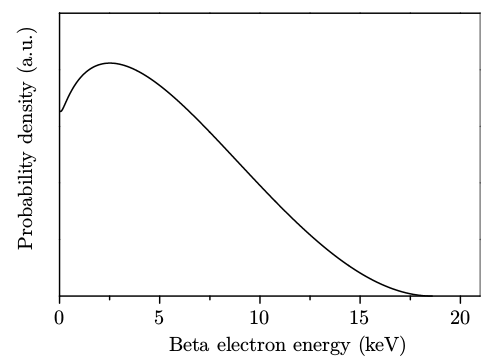
\includegraphics[scale=0.6]{Espectro.png}
\centering
\caption{Espectro energético de los electrones de la desintegración del tritio ~\cite{TesisTritio}\label{fig:Espectrotritio}}
\end{figure}

El espectro del tritio presenta la forma típica de un espectro energético de desintegración $\beta$, con una energía máxima de $18.6~\keV$, una energía promedio de $5.7~\keV$ y una moda (valor más probable) lígeramente inferior a la energía promedio, entorno a $4.5~\keV$. Con estos valores de energía podemos apreciar que la energía de radiación del tritio es la más pequeña observada hasta el momento en los isótopos. Como consecuencia, el electrón presentará un recorrido libre medio muy corto, del orden de $3-5~\mm$ en el aire y de $5-6~\mu m$ en un medio sólido~\cite{Isotopos}.

\subsection{Detección del tritio}

El problema que queremos estudiar  reside en que los mecanismos de detección y monitorización de tritio utilizados en la actualidad, en concreto en centrales nucleares, que será el objetivo final del detector que pretendemos desarrollar en el grupo experimental internacional denominado \textit{Tritium}, son métodos lentos o con un alto umbral de detección ~\cite{limiteMB, Limitetiempo, Limite}. 

%foto Tritium

Por ejemplo, entre los métodos más empleados actualmente en centrales nucleares, esta el método de detección  de centelleo líquido. Este es el método más indicado para la detección de partículas beta de energía muy pequeña porque, como ya se ha visto al analizar el espectro energético de los electrones de la radiación   $\beta$ del tritio, estos tienen un recorrido libre medio muy pequeño (del orden del $\milli\meter$ o $\micro\meter$, dependiendo del medio~\cite{Isotopos}). Dado que sólo se pueden medir (con una probabilidad aceptable) las emisiones que han tenido lugar a una distancia del detector inferior al recorrido libre medio, la forma más efectiva de conseguir que un mayor volumen de la fuente radiactiva contribuya a la señal y que un mayor volumen del detector se encuentre a una distancia adecuada de la fuente radiactiva, es disolviendo este detector con el líquido radiactivo (en nuestro caso agua tritiada), y ésto sólo se puede conseguir utilizando detectores líquidos de partículas beta, como el líquido centelleador. 
El método de centelleo líquido consiste en tomar una muestra del líquido radiactivo, agua tritiada en nuestro caso, diluirla (habitualmente al 50\%) con el líquido centelleador y medir los fotones emitidos por este líquido centelleador, a partir de los cuales podremos determinar los electrones emitidos por la muestra de agua tritiada y detectados por el líquido centelleador. Sin embargo, para ello se necesita tomar una muestra y llevarla al laboratorio para el correspondiente estudio. En resumen se trata de un proceso de detección de agua tritiada basado en métodos off-line que ralentizan la monitorización, dilatando el resultado hasta varios días desde la toma de la muestra. 

Tras cada análisis, la muestra de agua tritiada y líquido centelleador son inseparables y por tanto no reutilizables.  El líquido centelleador debe de ser tratado como residuo peligroso ya que, aunque el análisis desvele que el agua tritiada esta libre de tritio (presente una actividad suficientemente baja para ser tratada como material no radiactivo), el líquido centelleador  contiene tolueno y, por tanto, debe de ser desechado de acuerdo con el protocolo de residuos químicos peligrosos, y en particular no puede ser vertido al medio ambiente. También necesita operarios especializados manipulen estas muestras, poniendo en peligro su salud~\cite{gel}.

\subsection{Esquema del trabajo}

El objetivo final de \textit{Tritium}, sobre el cual tratará mi futura Tesis Doctoral, es desarrollar un detector de aguas tritiadas que permita realizar la monitorización del tritio \textit{in situ} en tiempo cuasi-real. Por tiempo cuasi-real entendemos una dilatación temporal máxima de 10 minutos desde la toma de la muestra (ya que se necesita un tiempo mínimo para poder discernir la señal del background, el cual dependerá, entre otras cosas, de la configuración del sistema de detección). Además, el prototipo desarrollado no necesitará de la presencia de personal especializado que intervenga en el proceso de monitorización de aguas tritiadas, agilizando y abaratando el método de monitorización, además de excluir posibles errores humanos. El método simplemente requerirá continuas calibraciones al cabo de un tiempo determinado para asegurar el correcto funcionamiento del dispositivo. 

La dificultad aquí residirá en conseguir extraer esta señal tan pequeña ($\backsim 1~\keV$) y tener estadística suficiente para poder discernirla del fondo radiactivo en un tiempo tan pequeño. El proyecto \textit{Tritium} pretende llegar a realizar detecciones en el límite de actividades de la muestra de agua tritiada entorno a $0.1$ o $1~\kilo\becquerel/\liter$, lo cual nos permitirá generar mensajes de alarma cuando la muestra supere el límite recomendado por la Comunidad Europea, $100\becquerel/\liter$. Los trabajos \textit{in situ} con configuraciones del detector similares (centelleador + fotosensor) realizados hasta la fecha que utilizan el concepto de tiempo real, sólo han conseguido obtener una señal en el límite del $\MeV/\liter$~\cite{TesisTritio} o incluso decenas de $\kilo\becquerel/\liter$~\cite{Rat}. Estos están basados principalmente en plásticos centelleadores y tubos fotomultiplicadores (PMT) a diferencia de nuestro experimento, que consta de fibras centelleadoras (que detectan la radiación beta del tritio y la convierten en fotones) y tubos fotomultiplicadores o fotomultiplicadores de silicio (que detectan estos fotones y los convierten en electrones que conformarán la señal del sistema). 

En mi opinión, el uso de fibras centelleadores es una mejor elección ya que presentan un mayor volumen activo con el que detectar el la radiación del tritio,  sin necesidad de utilizar líquido centelleador, el cual, como he mencionado anteriormente, produce residuos peligrosos, además del coste del líquido centelleador no reutilizable. Además, las fibras centelleadoras presentan un mayor abanico de posibilidades en cuanto a la elección de las distintas estructuras de las mismas. Nuestro experimento se centrará en la utilización de SiPM, ya que estos presentan una mayor eficiencia de fotodetección, aunque también contemplaremos el uso de PMT. 

Hay que tener en cuenta que existen diseños que logran llegar a límites del orden del Bequerelio en un tiempo de 3 minutos, aunque estos están basados en configuraciones totalmente distintas, como por ejemplo un sistema, formado por un láser y cavidades espectroscópicas en forma de anillo, en el cual se  busca la existencia de resonacias y  se relaciona las frecuencias a las que estas ocurren con la concentración de tritio presente en la muestra~\cite{Anillo}. Sin embargo, éste es un estudio totalmente diferente, ya que necesita de un acondicionamiento y control exhaustivo de las condiciones del sistema para el correcto funcionamiento del láser, encareciendo la construcción y mantenimiento del mismo y dificultando la implantación de éste en sitios como centrales nucleares, es decir, es una aplicación que no persigue un mismo fin. 

Para conseguir extraer una señal tan pequeña con la mayor eficiencia posible,  estudiaremos diversas configuraciones experimentales para conseguir obtener la más adecuada de acuerdo a nuestro objetivo experimental. Además, realizaremos detecciones en coincidencia, lo cual nos permitirá eliminar en gran medida el fondo radiactivo del experimento. Las configuraciones que pretendemos abarcar en el experimento son: 
\begin{itemize}
\item {}
Por un lado estudiaremos cual es la mejor elección de las estructuras de fibras centelleadores. Estudiaremos las ventajas y desventajas que presenta la utilización clads en las fibras (recubrimiento de la fibra centelleadora para evitar la fuga de fotones de centelleo y poder dirigir estos de manera ópticamente aceptable hasta el fotosensor). 
\item {}
Por otro lado estudiaremos cual es la mejor elección del fotosensor. Las posibilidades contempladas en el experimento serán SiPM o PMT. Veremos cual es más adecuado, ya que cada una presenta una serie de características mejores como la eficiencia de fotodetección (PDE) de los SiPM sobre la de los PMT pero otras tantas peores como la dependencia con la temperatura más acusada en los SiPM que en los PMT.
\end{itemize}

También se realizarán una serie de simulaciones del experimento previas al desarrollo del mismo utilizando el programa Geant 4, desarrollado por el CERN, con el objetivo de ver que es el que deberíamos esperar teóricamente de nuestros resultados. Estas simulaciones nos permitiran comparar nuestros resultados experimentales con los datos simulados para ver hasta que punto nuestro experimento dista del modelo teórico seguido, lo cual nos permitirá a su vez comprobar la fiabilidad de este modelo teórico y corregir posibles erratas del mismo. También nos permitirá ver que posibles modificaciones podemos realizar en el experimento para obtener un mejor resultado.


%foto valencia

Dividiremos este trabajo en seis partes:
\begin{enumerate}
\item{} En primer lugar se realizará un pequeño estudio sobre las fibras centelleadoras. Por un lado se determinará cual es la forma adecuada de actuar a la hora de manipular fibras centelleadoras, elemento más sensible de los utilizados en el experimento, presentando el procedimiento final de como preparar un haz de fibras centelleadoras con resultado opticamente aceptable. Por otro lado se utilizarán distintas estructuras de las mismas para ver cual nos permite obtener una señal del agua tritiada  más óptima. 

\item{} En segundo lugar realizaremos una calibración de los SiPM, paso fundamental antes de poder obtener cualquier medida del experimento. La finalidad de este paso es poder catalogar la magnitud de la medida del sistema que estamos obteniendo con este instrumento, algo fundamental en física. No se necesita realizar una calibración de los PMT, paso igualmente importante al anterior, ya que este trabajo fue realizado recientemente por otro componente del grupo.

\item{} En tercer lugar se describirá uno de las posibles configuraciones que serán estudiadas con el fin de determinar cual de estas es la más adecuada, desde el punto de vista del objetivo final de proyecto, para el diseño final del detector. Este también nos permitirá encontrar posibles fallos y mejoras que optimicen nuestro prototipo y que podrán ser utilizadas para el diseño final. En concreto la configuración que se estudiará esta formada por un haz de 35 fibras centelleadoras sin clad leidas por PMT. También se hablará, entre otras cosas, del proceso de llenado que tuvo que ser desarrollado para una realización segura del mismo además del los resultados obtenidos.

\item{} En cuarto lugar se presentarán las simulaciones realizadas con el programa de Geant4\cite{Geant4a,Geant4b,Geant4c}, programa desarrollado por el CERN capaz de realizar simulaciones muy detalladas de experimentos, principalmente de física de partículas. En este punto, se presentarán las simulaciones realizadas tanto para los prototipos como para posibles diseños finales. Esto nos permitirá ver las posibles mejoras que podemos incluir a nuestro experimento y en que puntos difieren  las simulaciones de los resultados obtenidos en los distintos experimentos de los prototipo.

\item{} En quinto lugar, se presentarán partes del experimento que queden inconclusas o inacabadas o puntos interesantes y que serán propuestos a futuros estudios que habrá que realizar durante la Tesis Doctoral. También se comentará brevemente el siguiente paso que pretenderemos realizar en el proyecto.

\item{} Se presentará un último punto donde se expondrán las conclusiones alcanzadas en el trabajo.

\end{enumerate}